\hypertarget{evfolyam-osztalyzatok-bizonyitvany}{%
\section{Évfolyam, osztályzatok,
bizonyítvány}\label{evfolyam-osztalyzatok-bizonyitvany}}

A Budapest Schoolban tanuló gyerekek saját tanulási célokat tűznek ki,
tanulnak, alkotnak, trimeszterenként frissítik a portfóliójukat,
mentorukkal és a szaktanárokkal értékelik haladásukat, és ha kell,
újraterveznek.

Saját céljaik vannak, és sokszor a saját céljaik eléréséhez maguknak
kell felállítaniuk követelményeket. „Ha pszichológus akarok lenni, akkor
emeltszintű biológia érettségit kell tennem. Ehhez a mai tudásom alapján
nekem legalább hetente két órát kell a felkészüléssel foglalkoznom.''
Egyféle elvárásrendszer azonban adott a gyerek és az iskola számára, és
ez a Nemzeti Alaptanterv elvárásrendszere.

\hypertarget{evfolyam}{%
\subsection{Az évfolyam}\label{evfolyam}}

A Nemzeti Alaptanterv tantárgyanként megadott \emph{elvárt tanulási
eredményekkel} határozza meg, hogy mit kell a gyerekeknek megtanulniuk
ahhoz, hogy a NAT szerint is haladni tudjanak az 1. évfolyamtól a 12.
évfolyamig. Az iskola feladata a gyerekeknek ebben a haladásban segíteni
és a haladást nyomonkövetni. A BPS-iskolákban egy gyerek akkor éri el
egy tantárgy adott évfolyamhoz tartozó követelményeit, ha a NAT által
megadott tanulási eredmények legalább 41\%-át teljesíti. Ha a gyerek
az adott évfolyamhoz tartozó minden tantárgy követelményeit elérte,
akkor léphet következő évfolyamra.

\begin{quote}
A BPS modell az évfolyamokra úgy tekint, mint egy
% \href{https://en.wikipedia.org/wiki/Experience_point}
{szerepjáték
nehézségi szintjeire}: akkor léphet egy gyerek a következő szintre, ha
az évfolyamhoz köthető tantárgyi tanulási eredményekből eleget
összegyűjtött.
\end{quote}

\hypertarget{tanulasi-eredmenyek-evfolyamokra-es-felevekre-bontasa}{%
\paragraph{Tanulási eredmények évfolyamokra és félévekre
bontása}\label{tanulasi-eredmenyek-evfolyamokra-es-felevekre-bontasa}}

A BPS modell ---~a Nemzeti Alaptantervvel összhangban~--- több esetben
több évfolyamot átívelő szakaszokra adja meg a tanulási eredményeket. Ha
egy pedagógiai szakasz $H$ hosszúságú, és arra a szakaszra a Nemzeti
Alaptanterv $N$ tanulási eredményt határoz meg, akkor a program évente
$N/H$ tanulási eredmény elérését tekinti célnak mind a
$H$ évben.

Például a \emph{magyar nyelv és irodalom} tantárgyból 136 tanulási
eredményt kell elérni az első négy évfolyamon, ezért a program a
gyerekek számára az első évfolyamra 136$/$4~=~35 tanulási eredményt
elérését tűzi ki.

\hypertarget{folyamatos-es-egyertelmu-haladas}{%
\paragraph{Folyamatos és egyértelmű
haladás}\label{folyamatos-es-egyertelmu-haladas}}

Mivel a BPS visszajelző rendszere folyamatos és rendszeres visszajelzést
szorgalmaz, ezért a gyerekek a tanév közben is „gyűjtik'' a tanulási
eredményeket a
portfóliójukba (\ref{portfolio}.~fejezet, \pageref{portfolio}.~oldal).
Ennek alapján tanév közben nemcsak a gyerek, hanem a tanárai és a családja is
mindig nyomon követhetik, hogy hol tart a gyerek, és mit kell tenni azért,
hogy a tanév végére elérje a az évfolyamhoz tartozó követelményeket.

\hypertarget{kevert-korosztaly-es-az-evfolyamok}{%
\paragraph{A kevert korosztályok és az
évfolyamok}\label{kevert-korosztaly-es-az-evfolyamok}}

A gyerekek a BPS-iskolákban sokszor vannak náluk fiatalabb vagy épp
idősebb gyerekekkel. Sokszor, sokféle csoportbontásban dolgoznak:
ugyanaz a két gyerek, aki együtt, egy csoportban tanul angolul,
lehet, hogy külön tanul matematikáról, mert teljesen máshol tartanak
a megértésben. Így az a kérdés, hogy \emph{„hányadikos vagy?''}, nem
annyira releváns a mindennapi tanulásban, mint az, hogy \emph{,,mit tanulsz épp?''}

\begin{figure}
\centering
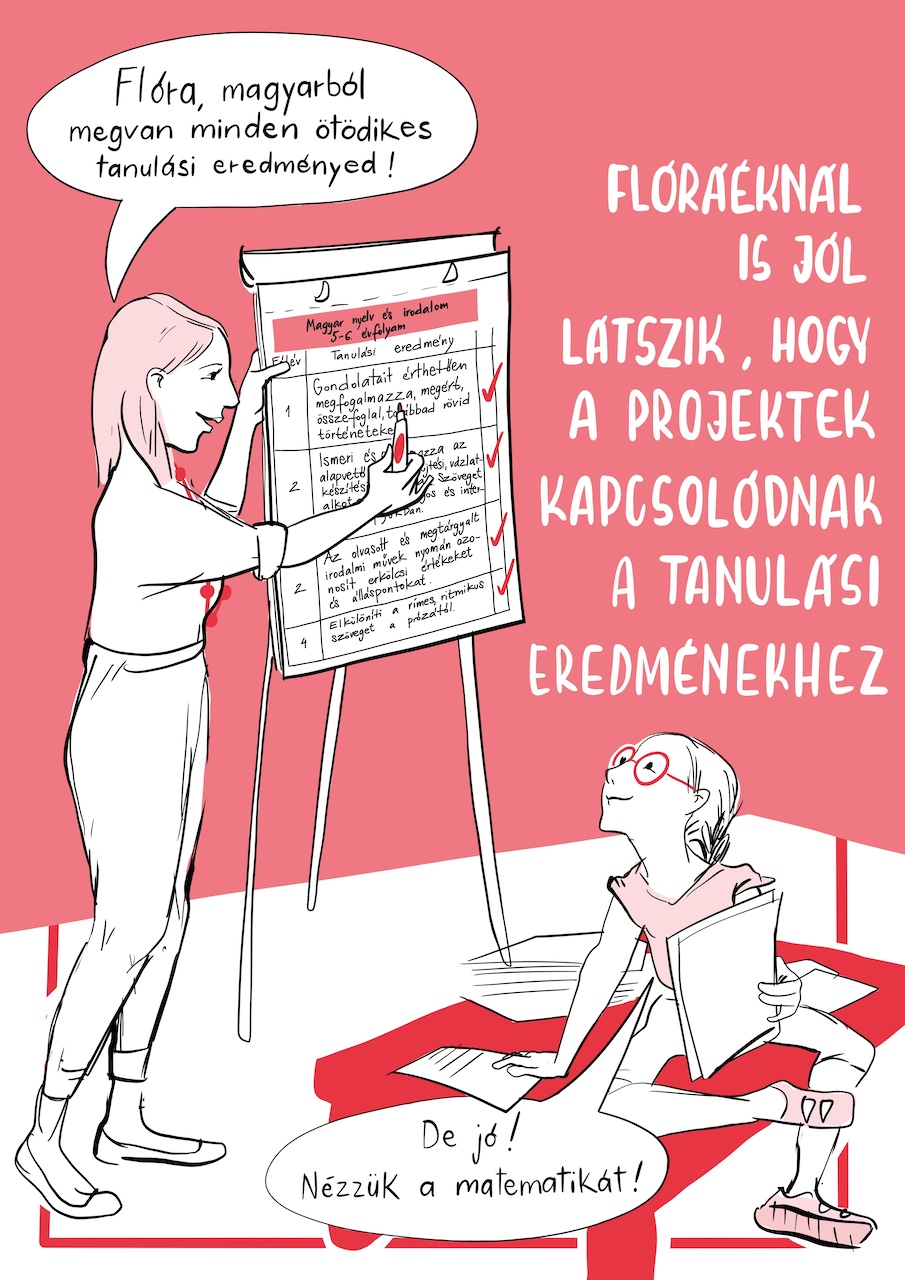
\includegraphics{pics/6b_tantargyi_flora.jpg}
\caption{Tanulási eredmények elszámolása}
\end{figure}

\hypertarget{erdemjegyek-es-osztalyzatok}{%
\subsection{Érdemjegyek és
osztályzatok}\label{erdemjegyek-es-osztalyzatok}}

Az Nkt.54.§ (1) szerint az érdemjegyek a tanév közben kapott 1--5 számok,
amik folyamatosan és rendszeresen értékelik a gyerek
\emph{teljesítményét és előmenetelét}.

A BPS modell folyamatos, többszempontú visszajelzést szorgalmaz, azaz
\emph{az érdemjegyek szerepét átveszik a többszempontú értékelő táblázatok
és visszajelzések}, illetve \emph{a tanulási eredmények elszámolása}. A
visszajelzésnek (\ref{visszajelzes-ertekeles}.~fejezet, \pageref{visszajelzes-ertekeles}.~oldal)
alaposnak, specifikusnak, többszempontúnak, a folyamatra fókuszálónak
kell lennie. Ezt a szerepet egy 1-től 5-ig terjedő skála önmagában nem
tudja ellátni.

\hypertarget{osztalyzatok-kialakitasa}{%
\subsubsection{Osztályzatok
kialakítása}\label{osztalyzatok-kialakitasa}}

Tantárgyankénti osztályzatok csak a NAT szerinti tantárgyi tudást,
teljesítményt és előmenetelt értékelhetik, és kizárólag a tanulási
eredmények elszámolásával alakulnak ki.

A gyerekek bármikor elérhetnek egy tanulási eredményt, aminek ténye
bekerül a portfóliójukba. Egy tanulási eredményt vagy teljesített a
gyerek, vagy nem, részben teljesíteni nem lehetséges. A teljesítés
igazolásának szabályait az iskola SZMSZ-e szabályozza.

Az elért tanulási eredmények osztályzatra váltásának a módja a
következő:

\begin{itemize}
\tightlist
\item
  Vesszük a félévben, illetve év végén a teljes évben elért tanulási
  eredmények számát, tehát a gyerek által az adott félévben\slash évben
  teljesített tanulási eredmények számosságát.
\item
  Ezt elosztjuk a BPS modell elvárt tantárgyi tanulási eredményeinek
  számával, és megszorozzuk 100-zal.
\item
  A kapott százalékos mutatót az alábbi táblázat alapján osztályzattá
  alakítjuk:
\end{itemize}

\begin{longtable}[]{@{}ll@{}}
% \toprule
\bfseries Teljesítmény &\bfseries Osztályzat\tabularnewline
\midrule
\endhead
0 - 40\% & 1\tabularnewline
41 - 50\% & 2\tabularnewline
51 - 60\% & 3\tabularnewline
61 - 70\% & 4\tabularnewline
71 - 100\% & 5\tabularnewline
\bottomrule
\end{longtable}

Az Ntk. előírja a tanuló magatartásának és szorgalmának
értékelését és minősítését. Ezt a gyerek mentora trimeszterenként
szövegesen vagy értékelő táblázatokban adja át.

\hypertarget{osztalyozo-vizsga}{%
\subsection{Osztályozó vizsga}\label{osztalyozo-vizsga}}

Az évfolyamok teljesítésének és az osztályzatok megítélésének folyamata a
gyerek évközi alkotásait, munkáját, teljesítményét tartalmazó
portfólió alapján történik, ezért a folyamat megfelel a
20/2012.(VIII.31.) EMMI-rendelet 64.~§ (1) azon elvárásának, hogy a
tanuló osztályzatait \emph{„évközi teljesítménye és érdemjegyei''}
alapján kell megállapítani, azzal a megkötéssel, hogy a BPS modell
elfogadja az érdemjegyeknél gazdagabb szöveges és értékelőtáblázat-alapú
visszajelzést.

Ha a portfólió alapján nem állapítható meg az évfolyamszintlépéshez és
az osztályzathoz szükséges tanulási eredmények megléte, akkor a
gyereknek ki kell egészítenie a portfólióját. Ez történhet akár egy
tudáspróbával vagy egy online teszttel is. Vagy el kell fogadnia, hogy
\emph{még} nem érte el a következő évfolyamszintre lépéshez szükséges
tanulási eredményeket.

Ugyancsak kiegészítendő a portfólió, ha igazolt vagy igazolatlan
mulasztások miatt az iskolában végzett munka nem volt elegendő az
elégséges portfólió-elemek összegyűjtésére. Ez azt is jelenti, hogy az
iskolának nem kell a fenti folyamattól, folyamatoktól eltérnie, csak a
portfóliót kell kibővíteni, vagy a gyereknek el kell
fogadnia, hogy \emph{még} nem érte el a következő évfolyamszintre
lépéshez szükséges tanulási eredményeket.

Ha a gyereket bármely okból felmentették a tanórai foglalkozásokon való
részvétel alól, akkor a 20/2012.(VIII.31.) EMMI-rendelet 64.~§ (2)
alapján osztályozóvizsgát kell tennie. Az iskolában az osztályozó vizsga
a tanulási eredmények vizsgakörülmények közötti igazolása.
